\chapter{Results and Evaluation}\label{chap:5}

This chapter compare the results obtained in each stage and how those results are supported to narrow down the research to find number of optimal thread pool for given program. In the early phases broader measurement metrics ( average latency, throughput, Standard deviation, average latency, Median latency, 99th percentile of latency, error rate ) were analyzed to compare  architectures. Some metrics  In later phases average latency (in milliseconds) is used as main metric to compare performance. Chapter 3 explains the these metrics in detail.

In the first phase following architectures were implemented,

\begin{itemize}
	\item Ballerina current architecture
	\item Increasing Ballerina scheduler thread pool size into 2 times and 4 times
	\item Removing Ballerina Scheduler thread pool
	\item Changing Netty layer worker thread pool as thread per connection model  (Netty \acrshort{OIO}) 
\end{itemize}

\section{Results comparison of different architectures}

\begin{figure}[htbp]
	\begin{center}
		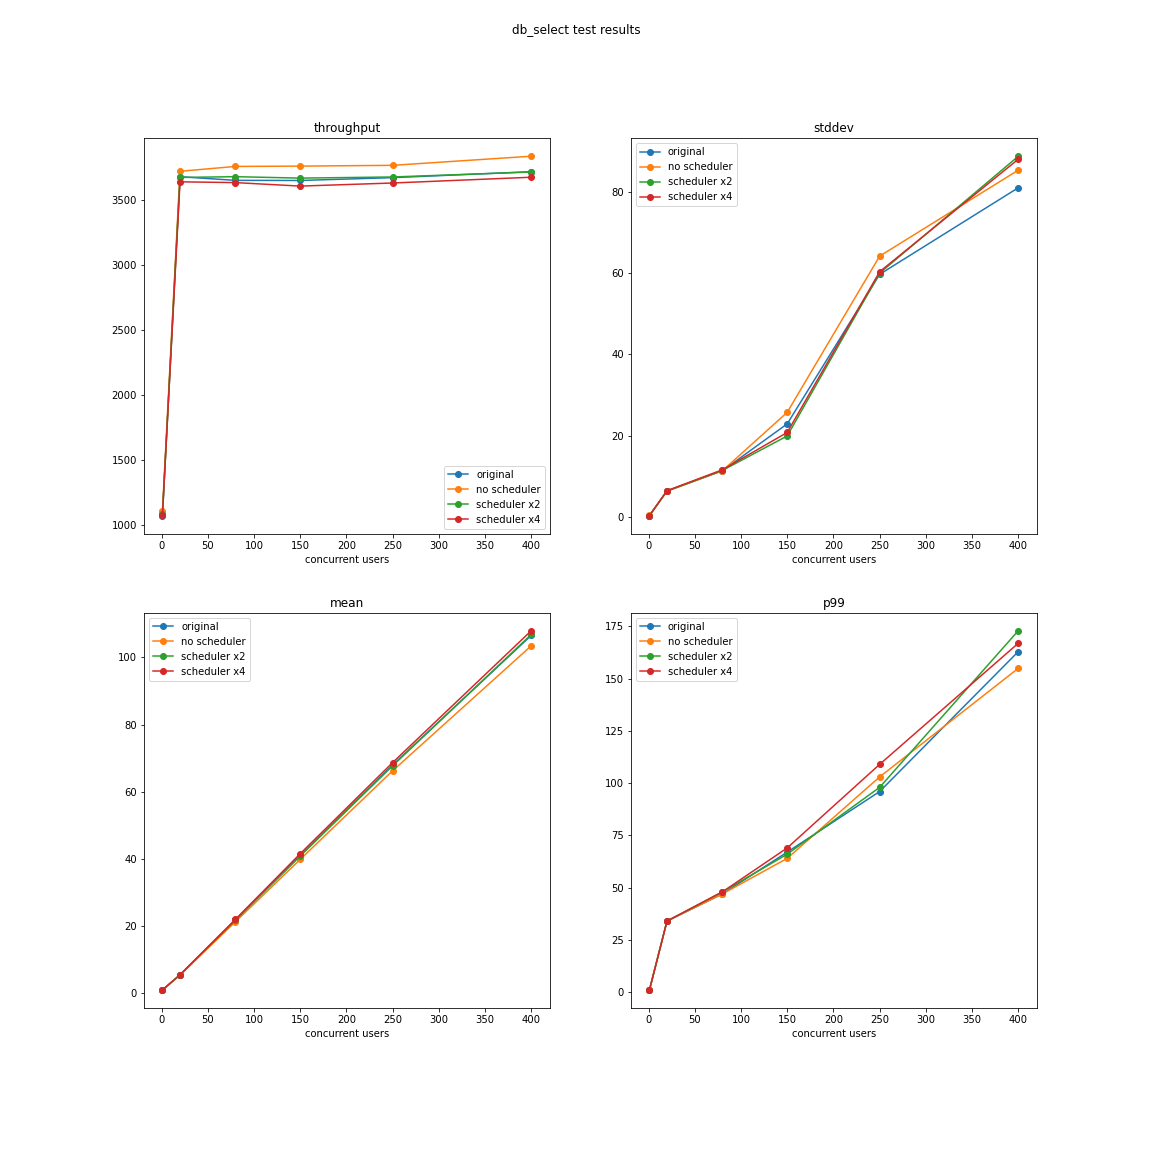
\includegraphics[scale=0.5]{figures/db_select test results.png}
	\end{center}
	\caption{Throughput, Avg. Latency(Mean), Standard deviation(stddev) and 99th percentile of latency  of Database call test for 1. Make twice the thread pool size of scheduler 2. Ballerina removing scheduler thread pool 3. Make 4 times the thread pool size of scheduler 4. Netty OIO architecture 5. Ballerina current architecture }
	\label{phase-1-database-all-architectures}
\end{figure}

\begin{figure}[htbp]
	\begin{center}
		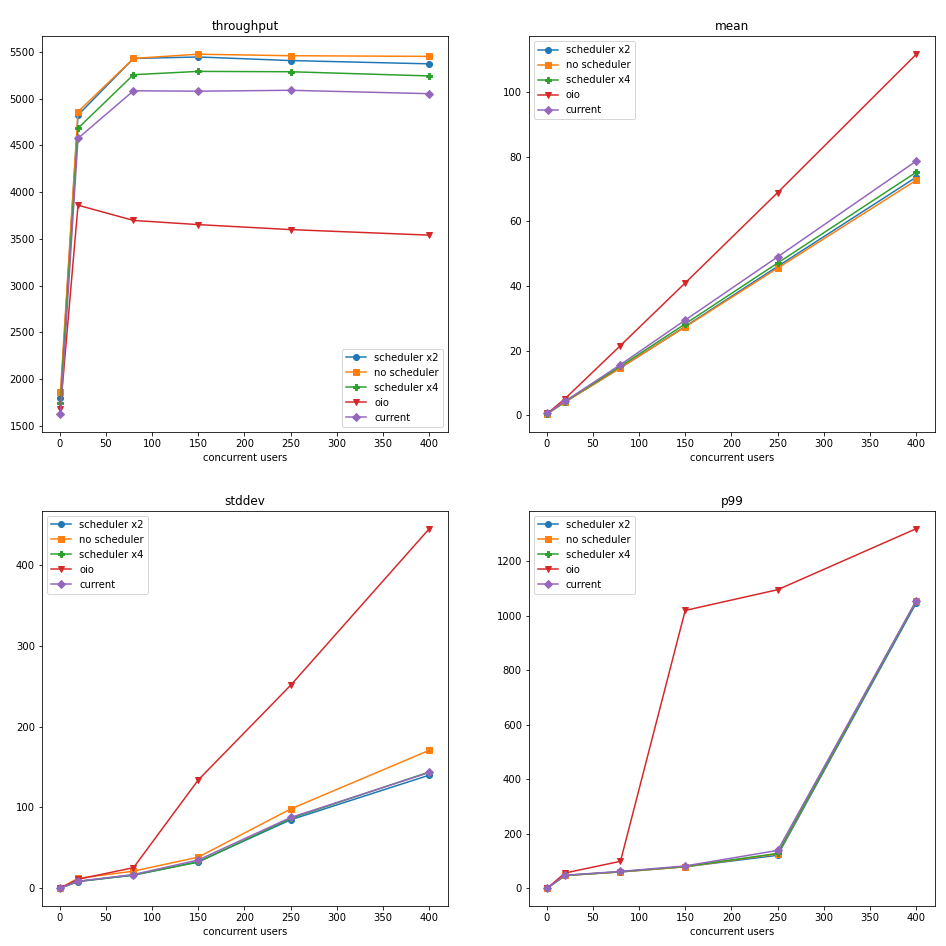
\includegraphics[scale=0.5]{figures/prime_small test results.png}
	\end{center}
	\caption{Throughput, Avg. Latency(Mean), Standard deviation(stddev) and 99th percentile of latency for Prime small test }
	\label{phase-1-prime-small-all-architectures}
\end{figure}

\begin{figure}[htbp]
	\begin{center}
		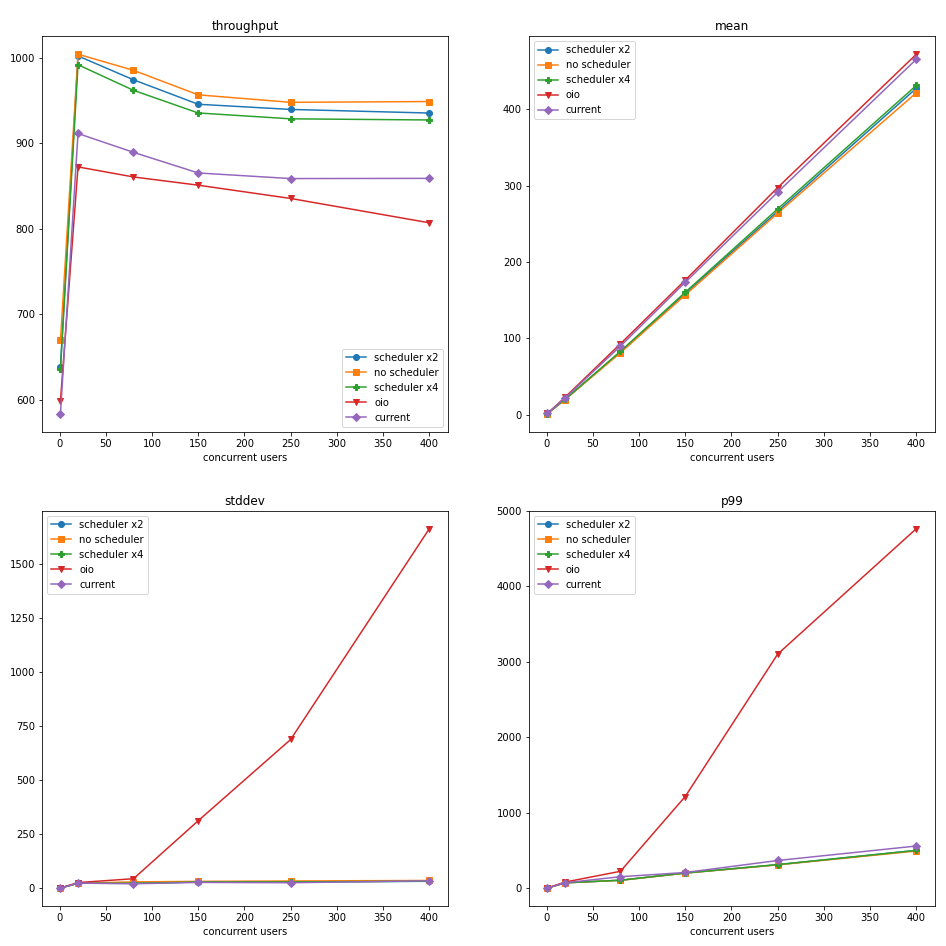
\includegraphics[scale=0.5]{figures/prime_medium test results.png}
	\end{center}
	\caption{Throughput, Avg. Latency(Mean), Standard deviation(stddev) and 99th percentile of latency for Prime medium test }
	\label{phase-1-prime-medium-all-architectures}
\end{figure}

\begin{figure}[htbp]
	\begin{center}
		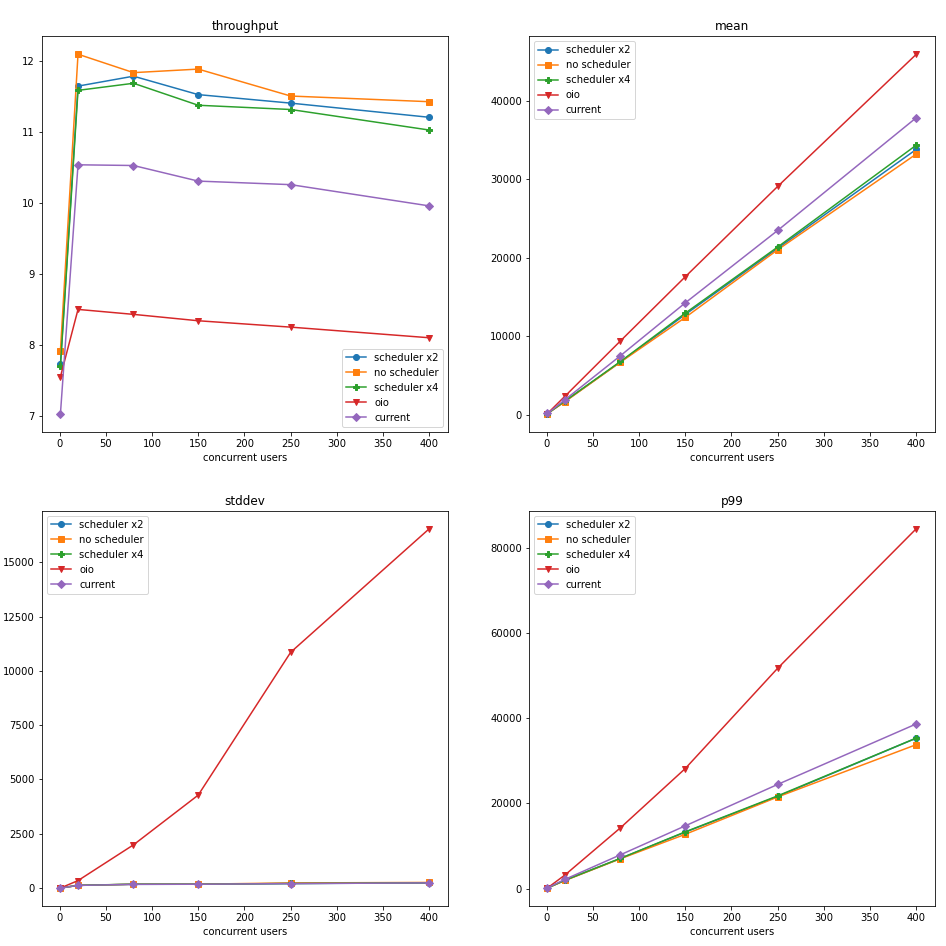
\includegraphics[scale=0.5]{figures/prime_large test results.png}
	\end{center}
	\caption{Throughput, Avg. Latency(Mean), Standard deviation(stddev) and 99th percentile of latency for prime large test }
	\label{phase-1-prime-large-all-architectures}
\end{figure}

\begin{figure}[htbp]
	\begin{center}
		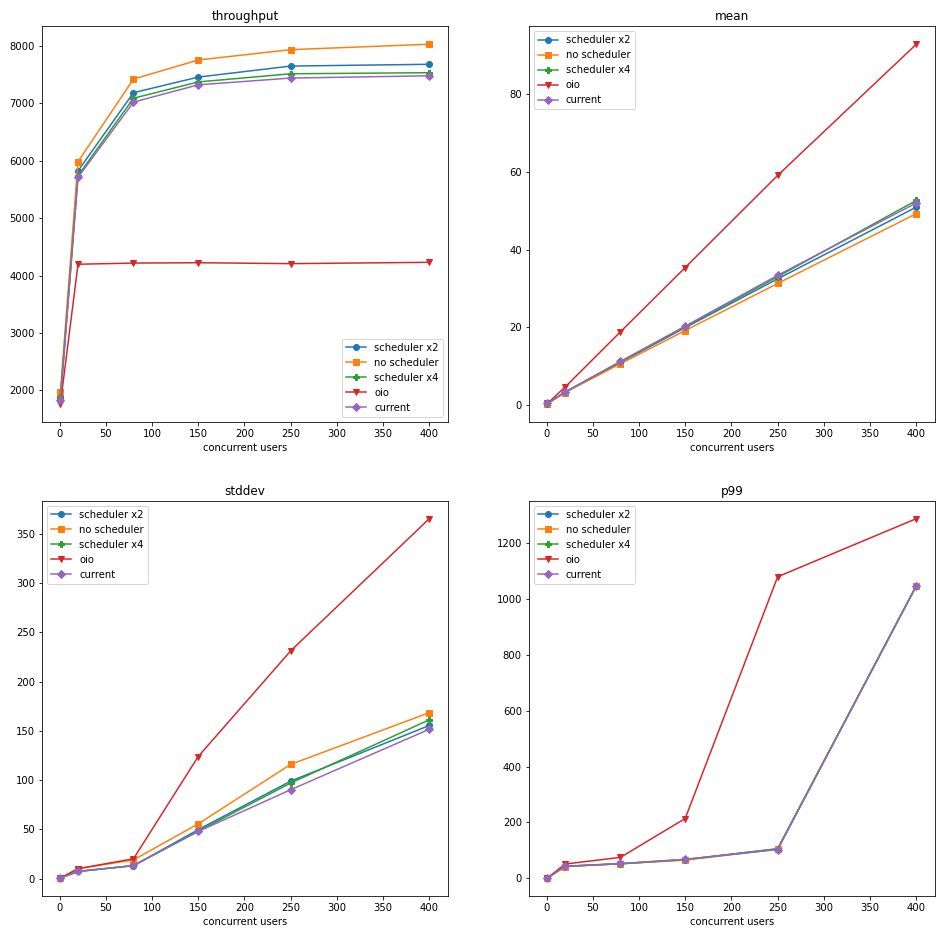
\includegraphics[scale=0.5]{figures/file test results.png}
	\end{center}
	\caption{Throughput, Avg. Latency(Mean), Standard deviation(stddev) and 99th percentile of latency for file read test  }
	\label{phase-1-file-read-all-architectures}
\end{figure}

Metrics such as error rate is not shown in the plots since those metrics are used to verify the validity of obtained results in intermediate steps. Performance tests were started with Current ballerina architecture, Removing ballerina scheduler thread pool and Netty OIO architecture. Since Netty OIO performance (High latency and low throughput) is lowest in every case, focus is moved to tread pools. Then the behavior is analyzed with adding more threads to scheduler thread pool. Figures \ref{phase-1-database-all-architectures},\ref{phase-1-prime-small-all-architectures},\ref{phase-1-prime-medium-all-architectures},\ref{phase-1-prime-large-all-architectures},\ref{phase-1-file-read-all-architectures}, shows the throughput and latency results for Database, Prime small,Prime medium,Prime large and File read. In mentioned graphs it can be seen that OIO architecture has the lowest throughput, the highest latency and higher standard deviation among all the other architectural changes for almost every concurrency level. After initial tests OIO architecture was not considered for future tests. 

Another significant indication that removing ballerina scheduler able to gain significant performance(Higher throughput and lower latency). That performance gain is independent form the program type. Thus,it was not possible to find distinct situations where a certain architecture would perform well for one program type while another architecture performs well for another program type. Although changing thread pool size affected differently in CPU bound(Prime test) and IO cases (Database test). Then the direction of server architecture tuning is focused on tread pool tuning. In this phase it is only changed two values of thread pool size. That is not sufficient to bring any conclusion.

\begin{figure}[htbp]
	\begin{center}
		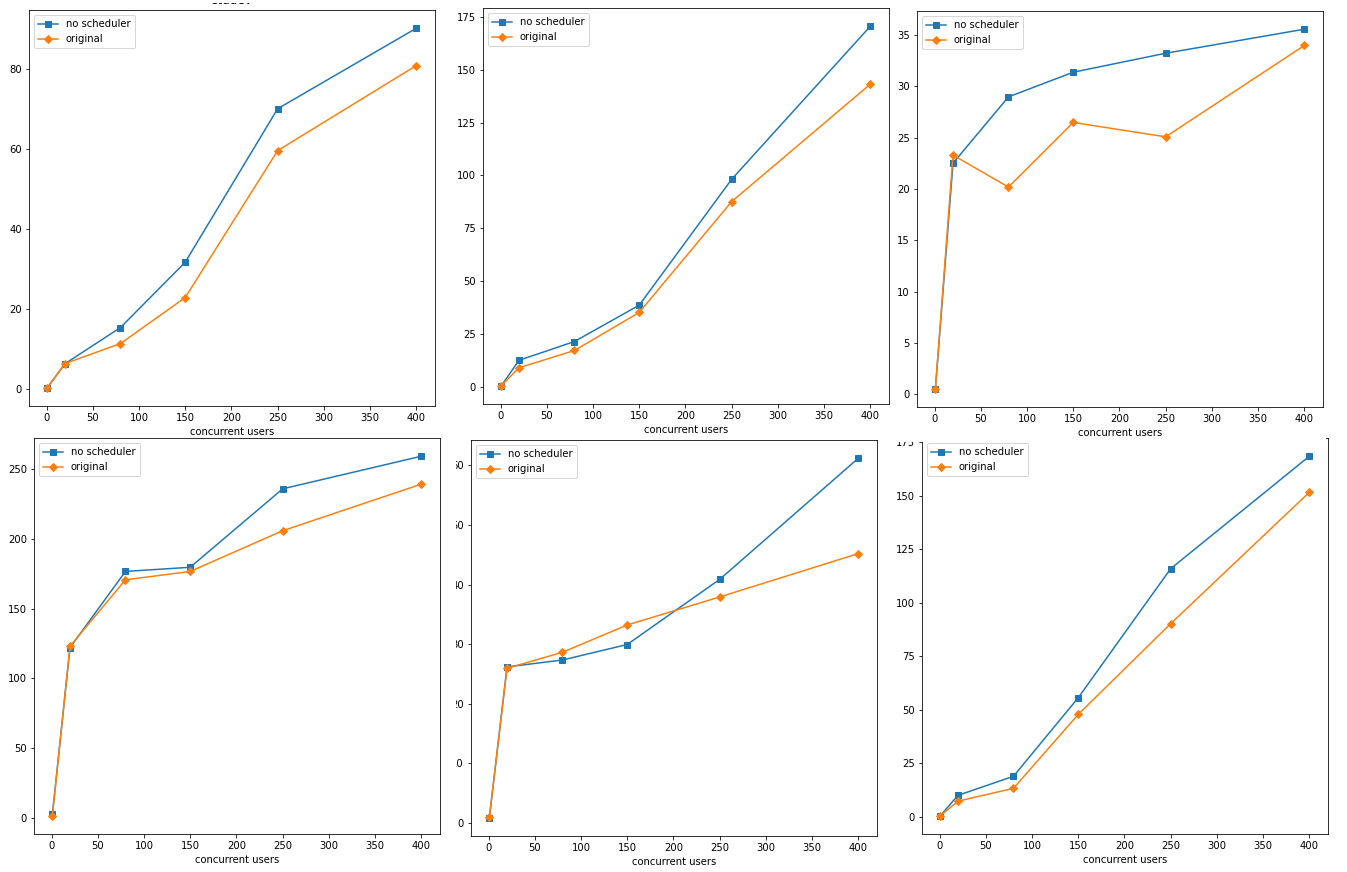
\includegraphics[scale=1.2]{figures/db-ps-pm-pl-ms-fr.png}
	\end{center}
	\caption{Standard deviation comparison of Database select test, Prime small test, Prime medium test, Prime large test, Prime medium test, Merge sort, File test }
	\label{all_sd}
\end{figure}


In order to evaluate the performance of sever architecture in depth standard deviation is another important metric. Although removing ballerina scheduler perform well by throughput and latency, standard deviation is higher than current ballerina architecture for every program type. Since OIO architecture has greater standard deviations, values are not clear in the above figures. To analyze more clearly Figure \ref{all_sd} shows standard deviation values for current architecture and removed scheduler architecture. It is clear that having Ballerina's scheduler thread pool provide more stable results. Also, it is noticeable that increasing thread pool size of the Ballerina scheduler thread pool able to decrease the average latency closer as removed Ballerina scheduler thread pool. There is a trade off between stability and latency when scheduler thread pool is removed. In order to maintain stability it is chosen to keep ballerina scheduler thread pool.

Test programs were designed to have CPU bound and IO bound features in order to evaluate which server architecture is better for IO bound programs and which architecture is better for CPU bound program. Results obtained in this phase does not able to differentiate performance of architecture based on program type. However, it is clear that changing the thread pool size affected differently in IO bound and CPU bound programs. When comparing the throughput of Database test case (Figure \ref{phase-1-database-all-architectures}) and Prime small test case (Figure \ref{phase-1-prime-small-all-architectures}), changing thread size affected most in the prime small test. In Database test, increasing thread pool size doesn't change the throughput and latency values significantly. The reason behind that scenario can be explained as, since database call is a blocking call which blocks the execution thread, two thread pool size variations ( 2 times and 4 times the default scheduler thread pool size) are not sufficient to gain significant performance different. Next experiments results are based on introducing more thread pool sizes to the ballerina scheduler considering results on this phase. Also, there is lack of programs based on IO features in the initial experiments even though there are many CPU intensive programs. Thus new IO programs are added to the experiments.

\section{Results comparison of different thread pool size}

\begin{figure}[htbp]
	\begin{center}
		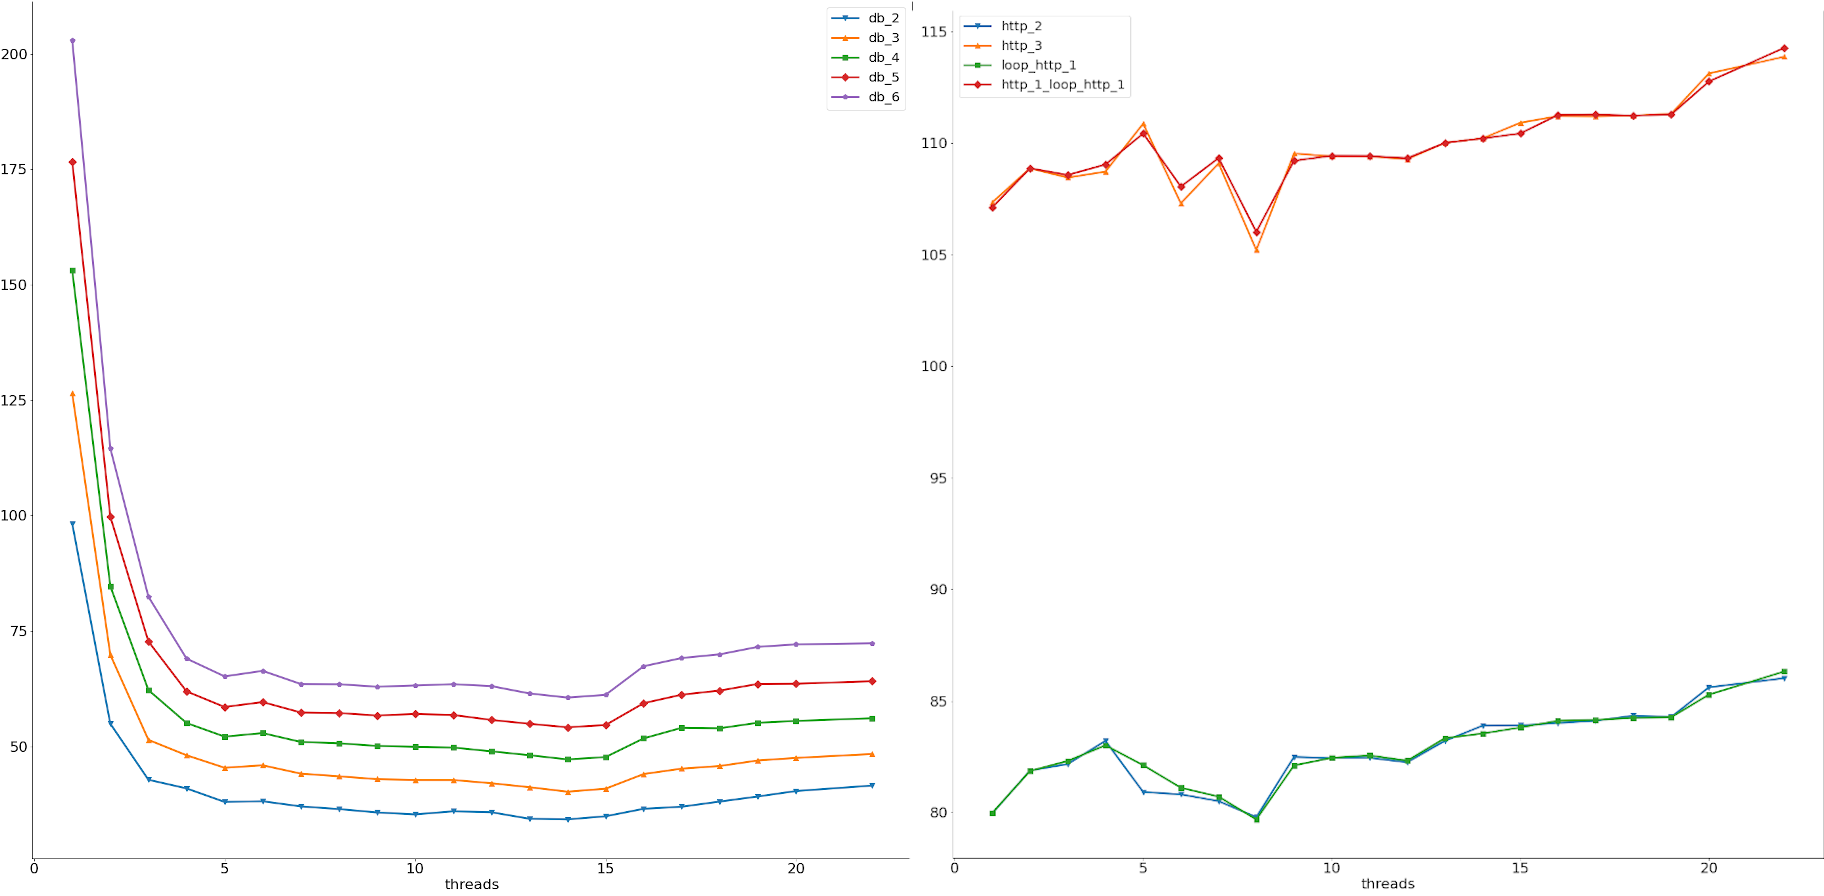
\includegraphics[scale=1]{figures/pool-db-http.png}
	\end{center}
	\caption{Left plot shows Thread pool size vs Average latency (millisecond) for number of database calls. \textbf{db\_2} represent program has 2 database calls. Right plot shows Thread pool size vs Average latency (millisecond) for number of http calls and number of loops which contains http calls}
	\label{thread_pool_database_and_http}
\end{figure}

\begin{figure}[htbp]
	\begin{center}
		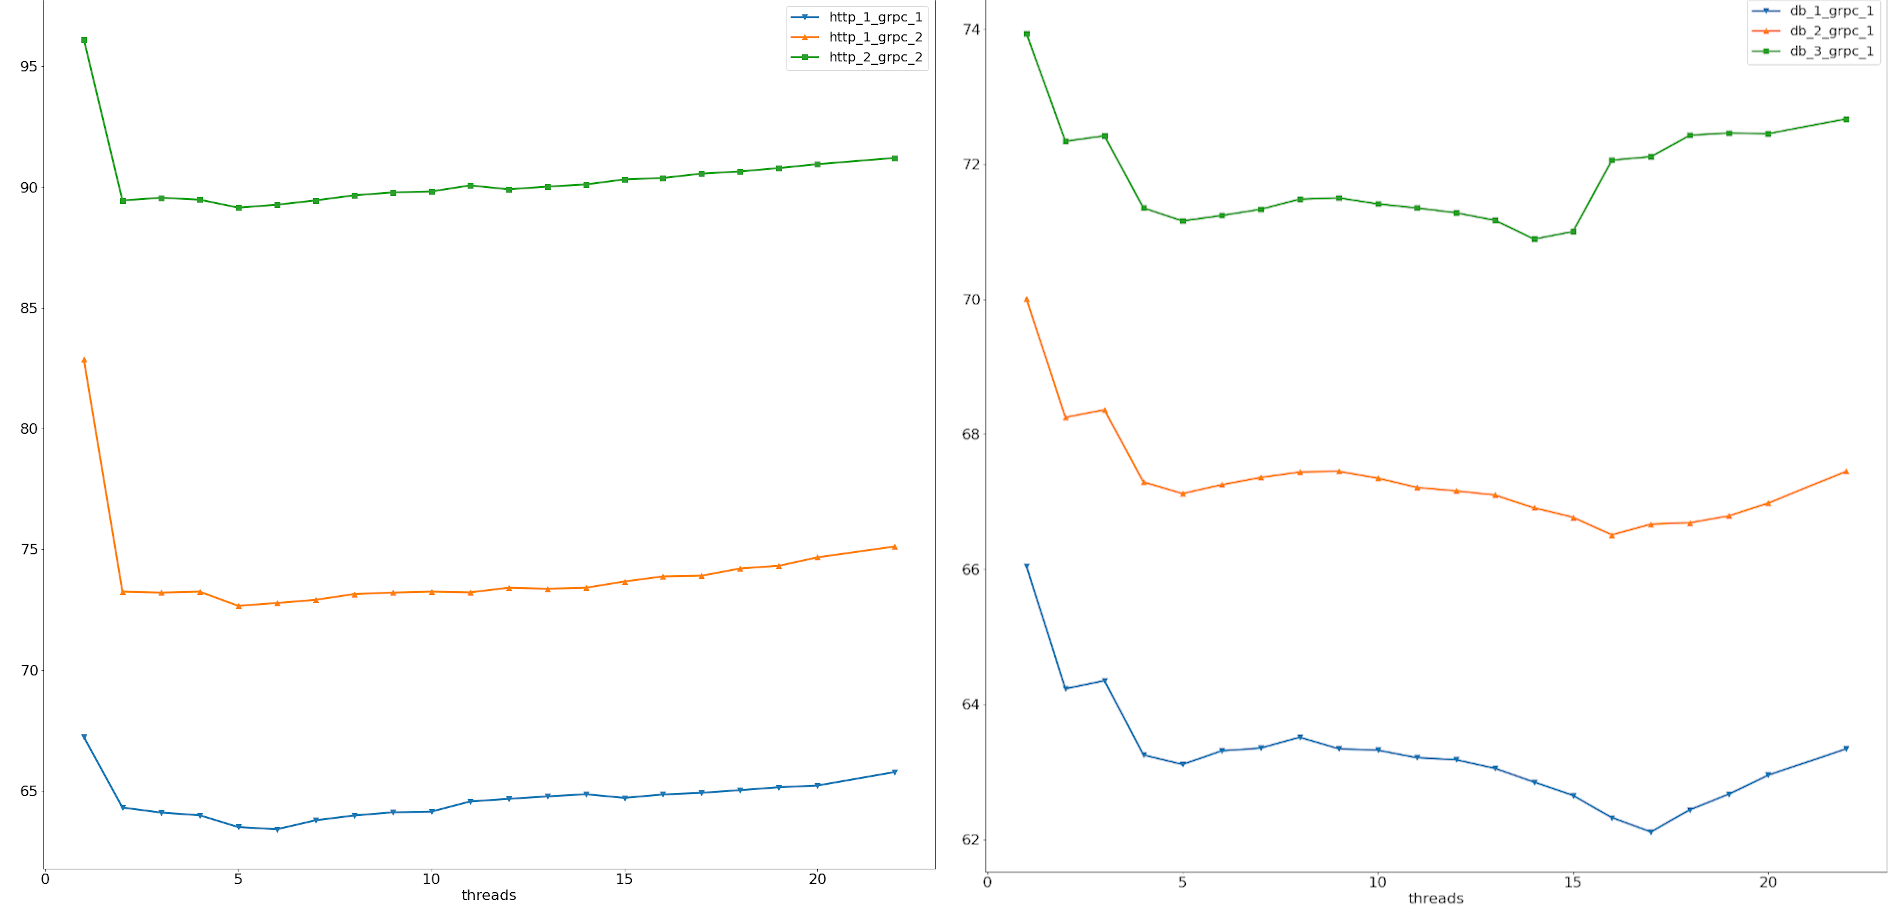
\includegraphics[scale=1]{figures/pool-http-db-db-grpc.png}
	\end{center}
	\caption{Left plot shows Thread pool size vs Average latency (millisecond) for number of database calls and grpc calls. \textbf{http\_1\_grpc\_2} represent that program has 1 http call and 2 grpc calls. Right plot shows Thread pool size vs Average latency (millisecond) for number of database calls and number of grpc calls.}
	\label{thread_pool_http_db_and_db_grpc}
\end{figure}

Based on previous experiment set, performance is evaluated for different thread pool sizes. Programs which contains different type of IO features are analyzed. In previous experiment sets for IO features,  there were only database call test. Programs with following IO features are evaluated,
\begin{itemize}
	\item gRPC calls
	\item Database calls
	\item HTTP calls
\end{itemize}

Implemented programs contains above IO features. This experiment is aimed to obtain to get thread pool size which gives the minimum latency. More details of the design is explained in chapter 3. Results are taken from  82 programs.

Figure \ref{thread_pool_database_and_http} and figure \ref{thread_pool_http_db_and_db_grpc} shows some results for thread pool size of 1 to 22. This range is selected because minimum of the average latency is always laid between this range. In order to verify the selected range, experiments are conducted for higher number of thread pool sizes. Those results showed only increase of average latency. 

From these experiments, thread pool size which gives minimum latency is obtained in order to feed the machine learning model. 

\section{Results comparison of machine learning models}

This section presents the results of machine learning models. The machine learning model can be expressed as follows,

$$ Optimal\:thread\:pool\:size = f(\:Program\:features)$$

After feature engineering steps, following features are selected to train the machine learning model.

\begin{itemize}
	\item Number of HTTP connector calls
	\item Number of Database connector calls
	\item Number of non-blocking gRPC connector calls
	\item Whether each type of connector calls lies inside a loop 
	\item Whether loops contain HTTP,Database or gRPCS calls (As separate features)
\end{itemize} 

Features are obtained by parsing the AST of Ballerina programs. Input of the training data set is above programming features and output is the optimal thread pool size which gives the minimum latency. Table \ref{tab:data_frame_with_results} shows the fragment of the data set.

\begin{figure}[htbp]
	\begin{center}
		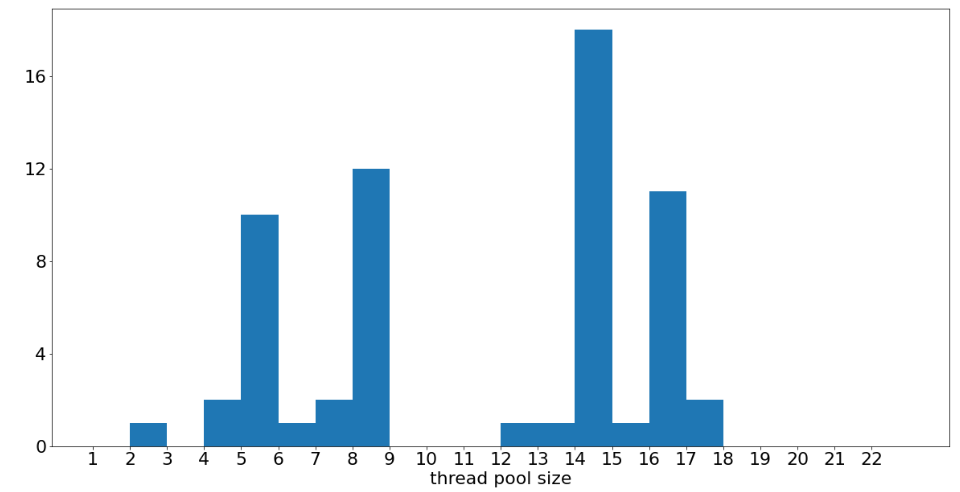
\includegraphics[scale=0.5]{figures/pool_size_dist.png}
	\end{center}
	\caption{No. of occurrences of optimal thread pool sizes.}
	\label{pool_size_dist}
\end{figure}

% Please add the following required packages to your document preamble:
% \usepackage{multirow}
\begin{table}[]
	\caption{Fragment of training data set}
	\label{tab:data_frame_with_results}
	\begin{tabular}{|l|l|l|l|l|l|l|}
		\hline
		\multirow{2}{*}{\textbf{Program}} & \multicolumn{5}{l|}{\textbf{Features}}                                                                                                                                                                                                                                                                                                                                                                    & \textbf{\begin{tabular}[c]{@{}l@{}}Optimal \\ thread \\ pool size\end{tabular}} \\ \cline{2-7} 
		& \textbf{\begin{tabular}[c]{@{}l@{}}No. of \\ database \\ calls\end{tabular}} & \textbf{\begin{tabular}[c]{@{}l@{}}No. of \\ HTTP \\ calls\end{tabular}} & \textbf{\begin{tabular}[c]{@{}l@{}}No. of\\ gRPC\\ calls\end{tabular}} & \textbf{\begin{tabular}[c]{@{}l@{}}No. loops \\ that contains\\ database \\ calls\end{tabular}} & \textbf{\begin{tabular}[c]{@{}l@{}}More \\ features...\end{tabular}} & \textbf{}                                                                       \\ \hline
		Program 1                         & 1                                                                            & 0                                                                        & 0                                                                      & 0                                                                                               & ...                                                                  & 14                                                                              \\ \hline
		Program 2                         & 1                                                                            & 2                                                                        & 0                                                                      & 0                                                                                               & ...                                                                  & 5                                                                               \\ \hline
		...                               & ...                                                                          & ...                                                                      & ...                                                                    & ...                                                                                             & ...                                                                  & ...                                                                             \\ \hline
	\end{tabular}
\end{table}

Then each following machine learning model is trained with the above data-set. The data set of 82 rows are relatively small. But there are other studies \cite{7459644,ahmed2015using} that used smaller data sets similar to this for Regression problems. Moreover, purpose of this research is to show a proof of concept that program features can be used to predict performance attributes.  

 In order to avoid over-fitting because of data set is small 5-fold cross validation is performed. For evaluation the performance of machine learning model 30\% of data is used as test data. Then following machine learning models are selected and evaluated the accuracy of each model.

This problem is originally a regression problem. But when it is analyzed the optimal thread pool size for each program, the distribution is very narrowed. Figure \ref{pool_size_dist} shows number of occurrences of each thread pool size. High frequency of optimal thread pool values can be seen around values of 5,8,14 and 16. Thus four classes can be created and reduce the machine learning model to classification problem as well. But there are some low frequency values around high frequency values also. For example around the value of 14, there are values of 12,13 and 15. Frequency of them is one. Those programs can be assigned to nearby class by observing the data set. Considering this fact results are shown for both classification and regression models. However, the accuracy of classification model is low compared to regression model. Results is presented in table \ref{tab:model-performance}.

\begin{itemize}
	
	\item XGBoost
	\item Support Vector Machine
	\item Decision Tree
	\item Random Forest
	
\end{itemize}


\begin{figure}[htbp]
	\begin{center}
		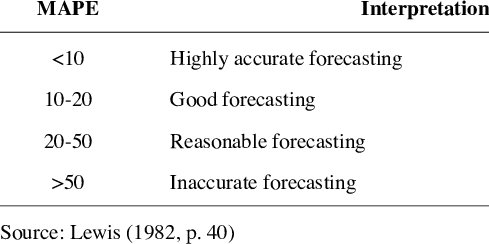
\includegraphics[scale=1]{figures/MAPE-values.jpg}
	\end{center}
	\caption{\acrfull{MAPE} Value interpretation for regression models}
	\label{MAPE_forcasting}
\end{figure}

For regression models \acrfull{MAPE} and \acrfull{MSE} are evaluated. For classification models F1 score and accuracy are evaluated. When comparing models, it is clear that Decision Tree Regression model has the lowest \acrfull{MAPE} and \acrfull{MSE} values. Lewis and Colin David \cite{lewis1982industrial} suggest ranges of MAPE values that provide insights on how good the forecasting. Figure \ref{MAPE_forcasting} shows the summary of MAPE value interpretation. Thus, Decision tree model has highly accurate forecasting of thread pool size for given set of programming features. Despite MAPE value is lower than Decision tree, XGboost and Random forest model falls under  highly accurate forecasting.

\begin{table}[]
	\caption{Evaluation of different machine learning model}
	\label{tab:model-performance}
	\begin{tabular}{|l|l|l|l|l|l|}
		\hline
		\multirow{2}{*}{\textbf{\begin{tabular}[c]{@{}l@{}}Machine \\ Learning\\ Model\end{tabular}}} & \multicolumn{3}{l|}{\textbf{Classification}}                                                                                                                 & \multicolumn{2}{l|}{\textbf{Regression}} \\ \cline{2-6} 
		& \textbf{Accuracy} & \textbf{\begin{tabular}[c]{@{}l@{}}F1 score\\ macro\end{tabular}} & \textbf{\begin{tabular}[c]{@{}l@{}}F1 score\\ weighted\end{tabular}} & \textbf{MAPE}        & \textbf{MSE}      \\ \hline
		XGBoost                                                                                       & 62.73\%           & 59.38\%                                                           & 62.29\%                                                              & 7.92\%               & 0.91              \\ \hline
		SVM                                                                                           & 59.09\%           & 45.08\%                                                           & 52.97\%                                                              & 30.06\%              & 13.41             \\ \hline
		\textbf{Decision Tree}                                                                        & 66.36\%           & 62.93\%                                                           & 67\%                                                                 & \textbf{6.79\%}      & \textbf{0.91}     \\ \hline
		Random Forest                                                                        		  & 68.59\%           & 61.58\%                                                           & 69\%                                                                 & 9.17\%      & 1.55\%     \\ \hline
	\end{tabular}
\end{table}

\section{Result evaluation of Machine learning model prediction vs Current Ballerina architecture}

\begin{figure}[htbp]
	\begin{center}
		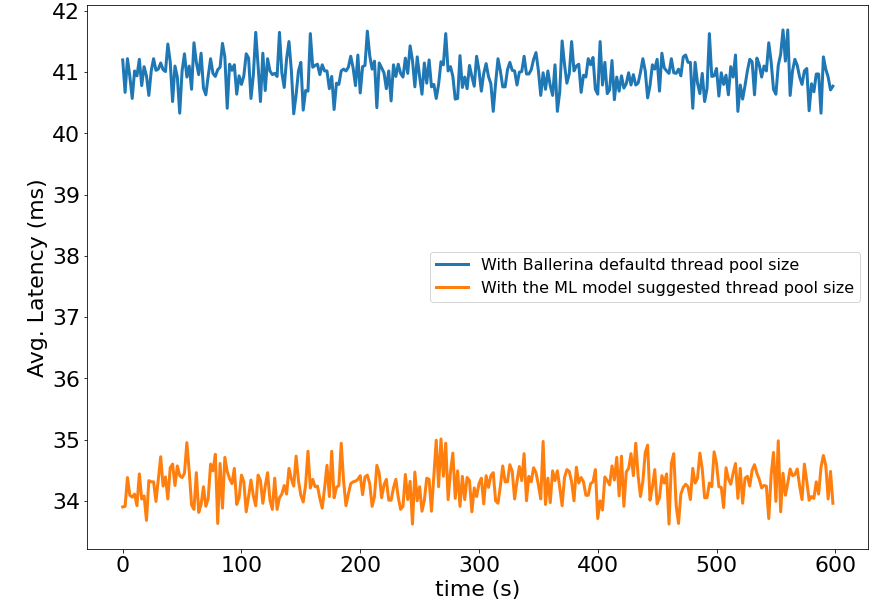
\includegraphics[scale=0.5]{figures/ts_db_2.png}
	\end{center}
	\caption{Program 1: consist of 2 database calls }
	\label{ts_db_1}
\end{figure}

\begin{figure}[htbp]
	\begin{center}
		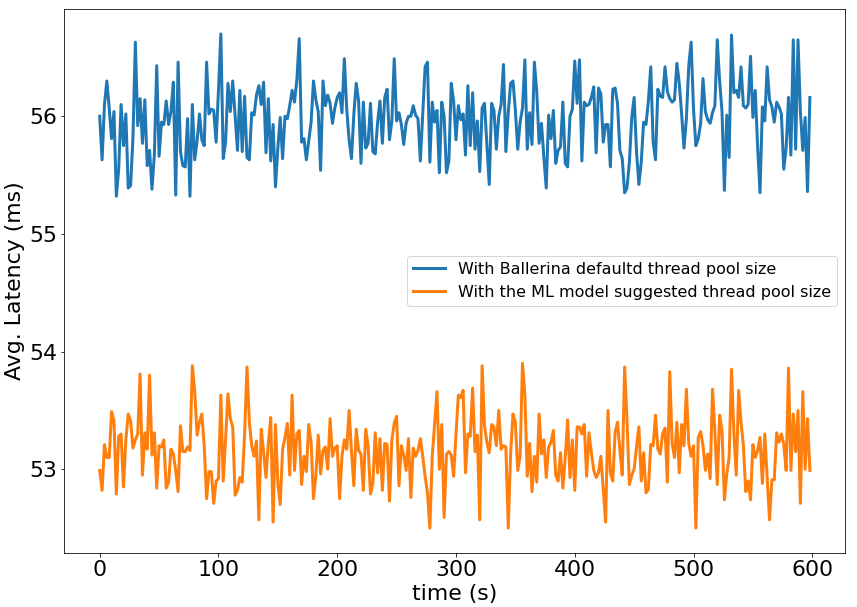
\includegraphics[scale=0.5]{figures/ts_http_1.png}
	\end{center}
	\caption{Program 2: consist of 1 HTTP call}
	\label{ts_http_1}
\end{figure}

In order to show how well the predicted thread pool size from the machine learning model improve the performance over default thread pool size, the Ballerina server was run under default thread pool size and thread pool size estimated by the Machine learning model for each program for 10 minutes. Ballerina default thread pool size is considered as baseline. Then average latency is recorded in each 2 second time interval plotted as a time series. Figure \ref{ts_db_1} visualize a program which consist of 2 database calls. Figure \ref{ts_http_1} visualize a program which consist of 1 HTTP call. Time series data shows the accuracy of data for an extended period of time not at a single point. Results show that the thread pool size suggested by the machine learning model provides the lowest average latency for both programs.

\section{Conclusion}

First off, results were compared with different server architectures which are Netty OIO, Current Ballerina architecture, Removed Ballerina scheduler architecture and 2 thread pool size variations in Ballerina scheduler thread pool. Thereafter, results of various thread pool sizes in the Ballerina scheduler thread pool are compared against different programs which have different IO characteristics. Then different programs gave different thread pool sizes which result in minimum average latency. This is called optimal thread pool size for a given program. Afterward, the machine learning model is trained with different program features and corresponding optimal thread pool size. Results show that the Decision tree regression model is the best suit for this. Finally,  2 programs were run under the default Ballerina scheduler thread pool size and the ML model suggested thread pool size. Average latency was plotted as time series. It showed that predicted thread pool size from the machine learning model gave the lowest average latency for both programs. 
